\documentclass[a4paper, 11pt]{report}
\usepackage{blindtext}
\usepackage[T1]{fontenc}
\usepackage[utf8]{inputenc}
\usepackage{titlesec}
\usepackage{fancyhdr}
\usepackage{geometry}
\usepackage{fix-cm}
\usepackage[hidelinks]{hyperref}
\usepackage{graphicx}
\usepackage{titlesec}
\usepackage{caption}
\usepackage{subcaption}

\usepackage[english]{babel}

\geometry{ margin=30mm }
\counterwithin{subsection}{section}
\renewcommand\thesection{\arabic{section}.}
\renewcommand\thesubsection{\thesection\arabic{subsection}.}
\usepackage{tocloft}
\renewcommand{\cftchapleader}{\cftdotfill{\cftdotsep}}
\renewcommand{\cftsecleader}{\cftdotfill{\cftdotsep}}
\setlength{\cftsecindent}{2.2em}
\setlength{\cftsubsecindent}{4.2em}
\setlength{\cftsecnumwidth}{2em}
\setlength{\cftsubsecnumwidth}{2.5em}

\titlespacing\section{0pt}{12pt plus 4pt minus 2pt}{0pt plus 2pt minus 2pt}
\titlespacing\subsection{0pt}{12pt plus 4pt minus 2pt}{0pt plus 2pt minus 2pt}

\begin{document}
\titleformat{\section}
{\normalfont\fontsize{15}{0}\bfseries}{\thesection}{1em}{}
\titlespacing{\section}{0cm}{0.5cm}{0.15cm}
\titleformat{\subsection}
{\normalfont\fontsize{13}{0}\bfseries}{\thesubsection}{0.5em}{}
\titlespacing{\section}{0cm}{0.5cm}{0.15cm}

%=============================================================================

\pagenumbering{Alph}
\begin{titlepage}
\begin{flushright}

\includegraphics[width=4cm]{USyd}\\[2cm]
\end{flushright}
\center 
\textbf{\huge INFO1111: Computing 1A Professionalism}\\[0.75cm]
\textbf{\huge 2023 Semester 1}\\[2cm]
\textbf{\huge Self-Learning Report}\\[3cm]

\textbf{\huge Submission number: 2}\\[0.75cm]
\textbf{Github link: \url{https://github.com/zliu6203/SelfLearning}}\\[2cm]

{\large
\begin{tabular}{|p{0.35\textwidth}|p{0.55\textwidth}|}
	\hline
	{\bf Student name} & Zhili Liu\\
	{\bf Student ID} & 520451407\\
	{\bf Topic} & PyGame\\
	{\bf Levels already achieved} & X\\
	{\bf Levels in this report} & B\\
	\hline
\end{tabular}
}
\thispagestyle{empty}
\end{titlepage}
\pagenumbering{arabic}


%=============================================================================

\tableofcontents

%=============================================================================

\newpage
\section*{Instructions}

\textbf{Important}: This section should be removed prior to submission.

You should use this \LaTeX\ template to generate your self-learning report. Keep in mind the following key points:
\begin{itemize}
	\item \textbf{Submissions}: There will be three opportunities during the semester to submit this report. For each submission you can attempt 1 or 2 levels. Each submission should use the same report, but amended to include new information.
	\item \textbf{Assessment}: In order to achieve level B, you must first have achieved level A, and so on for each level up to level D. This means that we will not assess a higher level until a lower level has been achieved (though we will review one level higher and give you feedback to help you in refining your work).
	\item \textbf{Minimum requirement}: Remember that in order to pass the unit, you must achieve at least level A in the self-learning (unless you achieve level B in both the skills and knowledge categories).
	\item \textbf{Using this template}: When completing each section you should remove the explanation text and replace it with your material.
	\item \textbf{Referencing}: You should also ensure that any resources you use are suitably referenced, and references are included into the reference list at the end of this document. You should use the IEEE reference style \cite{usyd2} (the reference included here shows you how this can be easily achieved).
\end{itemize}


%=============================================================================


\newpage
\section{Level A: Initial Understanding}
\vspace{5mm}
\subsection{Level A Demonstration}
The three things that demonstrate my understanding for this topic are:
\begin{itemize}
	\item Make a successful window for PyGame including some screen elements (sprites).
	\item Using sound libraries.
	\item Responding to user input.
\end{itemize}

\subsection{Learning Approach}
I approached my learning by looking for the latest tutorials online with PyGame, specifically the ones with project examples. I browsed both video and website tutorials including official documentation for many new methods and modules to build a successful game using the PyGame module of Python.

Experimentation was my main method of learning; testing all the different built-in libraries of methods and objects including sprites ("draw" module), sounds ("mixer" module), and the window itself ("display" module). I self-learnt by using previous knowledge of game development in C\# and Java to my advantage - scenes, object priority, using external files etc. Additionally, I also used knowledge of window composition via WinForms and Tkinter.

\subsection{Challenges and Difficulties}
Due to the new syntax it was difficult to correctly load a window at all with the limited knowledge. The most difficult to learn was the while loop that the game is running on; it also contains a for loop which did not make much sense. I simply accepted it as fact instead of fully understanding it.

Even after the window was created, it was even more difficult to find any sprites to fill the window as opposed to Tkinter or WinForms, where sprites and screen elements were ready for use. Furthermore, PyGame did not include any built-in sound files and so sound effects \& music must be found online or created locally.


\subsection{Learning Sources}
\begin{tabular}{|p{0.45\textwidth}|p{0.45\textwidth}|}
	\hline
	Learning Source & Contribution to Learning\\
	\hline
	\href{https://www.pygame.org/wiki/tutorials}{Wiki tutorial} & Understanding what each module does and its methods and objects.\\
	\hline
	\href{https://www.youtube.com/watch?v=jO6qQDNa2UY}{Beginner video tutorial} & Understanding the basics of every major aspect of PyGame.\\
	\hline
	\href{https://www.pygame.org/docs/ref/mouse.html}{Official documentation (mouse input)} & Finding each method and the parameters necessary for these methods.\\
	\hline
	\href{https://opensource.com/article/20/9/add-sound-python-game}{Sound help} & Understanding how sound works and how to implement sound at an appropriate time.\\
	\hline
	\href{https://www.youtube.com/watch?v=YDP1Hk7uZFAs}{Another video tutorial for shapes} & Understanding what to do in the absence of assets with sprites.\\
	\hline
\end{tabular}
\\
\\
\subsection{Application artifacts}
In level A, I made a very simple program in PyGame demonstrating that a successful window (1280x720) is opened with some screen elements (background, red line, blue player square). The blue square is responding to user input by following the coordinates of the mouse and not allow the mouse to go past the red line or the screen. When the cube touches the red line, a sound effect is played exactly once. This is demonstrated in this diagram.

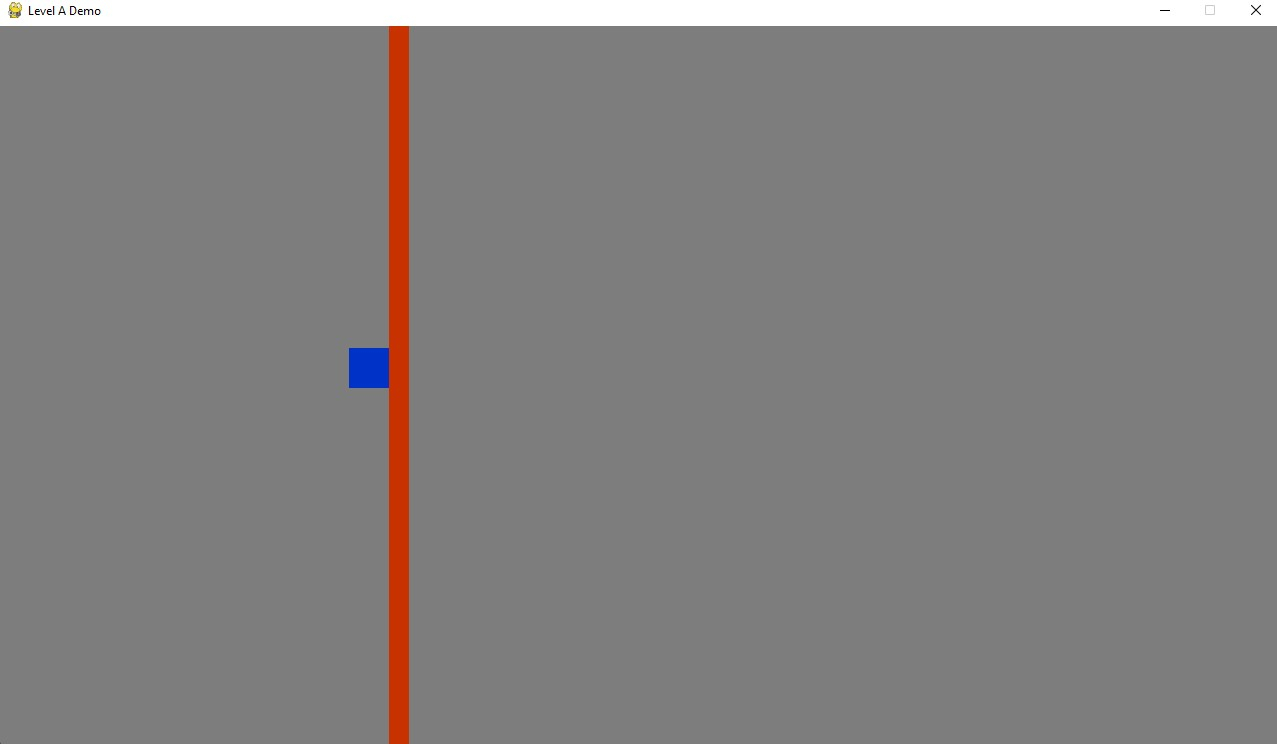
\includegraphics[width=8cm]{Level A Demo}\\[1cm]
\\
In the code, I used simple python syntax with some new PyGame methods and elements. In the follwing screengrabs, I showed this by using the main function and setting initial variables.

\begin{figure}[!htb]%
    \centering
    \subfloat[\centering Code showing variables]{{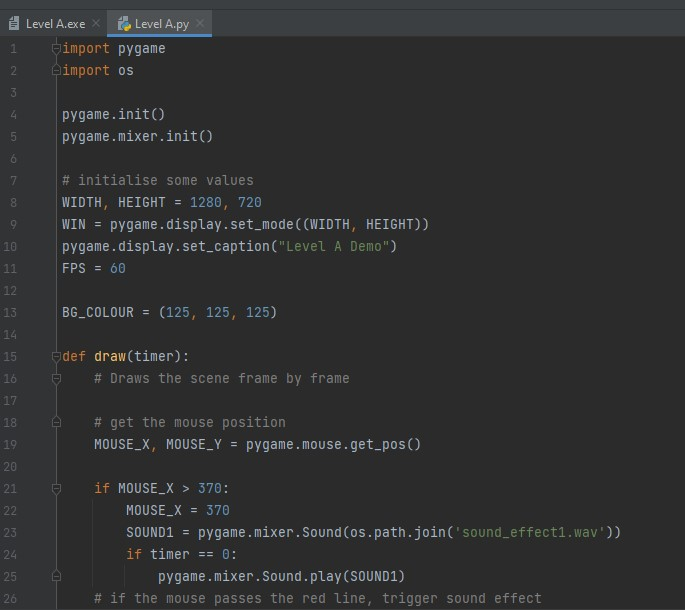
\includegraphics[width=6.5cm]{Level A Demo Code1} }}%
    \qquad
    \subfloat[\centering Code showing main function]{{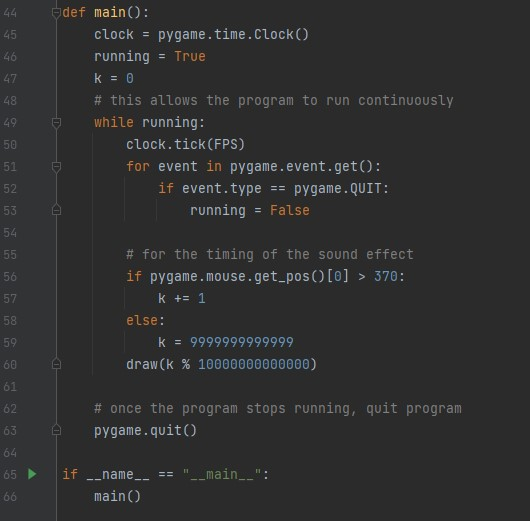
\includegraphics[width=6.5cm]{Level A Demo Code2} }}%
\end{figure}

Additionally, I used a simple sound effect from the web (sound\_effect1.wav) to play whenever the player hits the red line. I also used pyinstaller to make the .py into a .exe which is also included in the Git repository.

%=============================================================================

\newpage
\section{Level B: Basic Application}

Whilst level A is about doing something simple with the topic to just show that you have started to be able to use the tool or technology, level B is about doing something practical that might actually be useful.

\subsection{Level B Demonstration}

The application I have developed is a simple game in PyGame. This involves the three points in the level B proposal: events such as scenes, making a simple game with an end goal (win/lose), and program simple enemies. I have demonstrated the first point by making different levels in the game, satisfied the second point by creating a game with a goal (to finish all 5 levels), and also programmed simple enemies with random movement and bouncing back from the screen if it goes offscreen.

\subsection{Application artifacts}

I have created a simple topdown shooter game using built-in assets, modules, and tools only. The game I have made is simple: shoot all enemies using a periodic laser which can destroy all enemies collided with the laser. I used classes and small aspects of object oriented programming to achieve this.

In the following screengrab, the player can shoot a laser which only fires when the left mouse button is pressed and the cooldown for the laser is done. This laser collides with all enemies within its vicinity and destroys them. The player in blue and white can be controlled using WASD and the laser is shot in the direction of the cursor.
\\
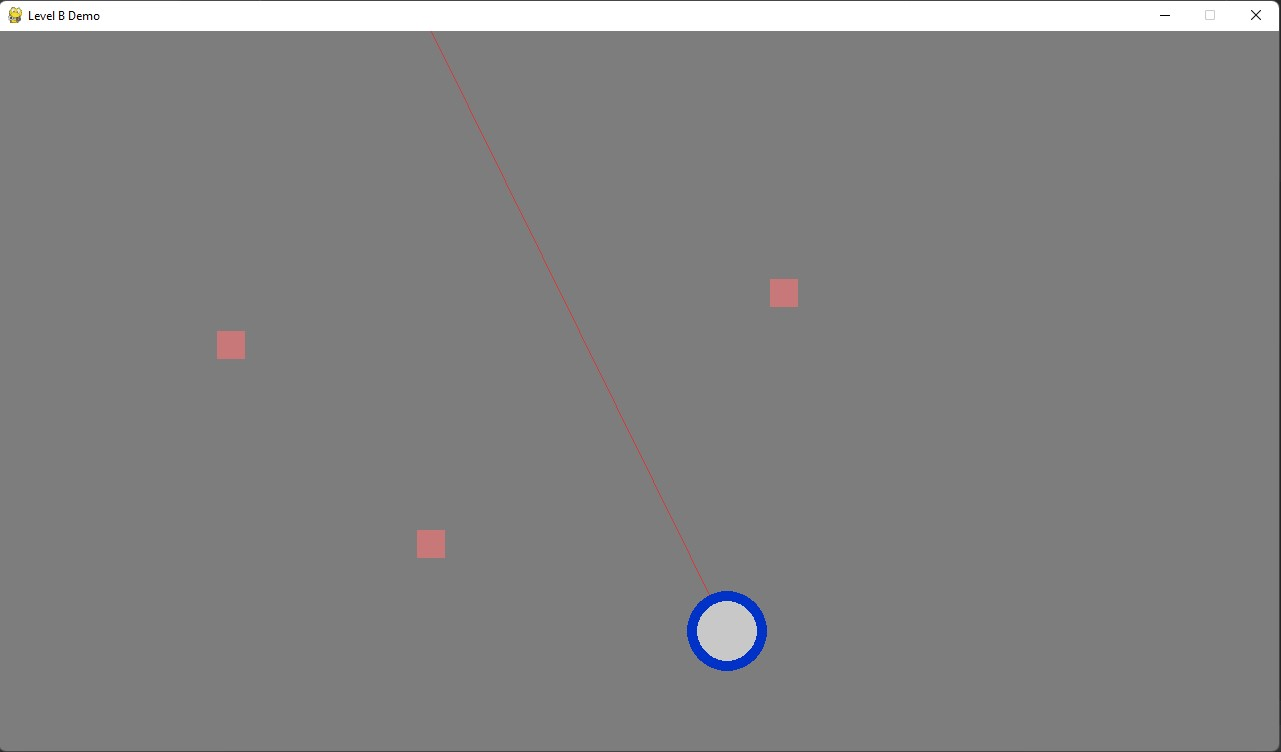
\includegraphics[width=8cm]{Level B Demo}\\[1cm]
\\

This screengrab shows the huge number of enemies in level 4 of this game:
\\
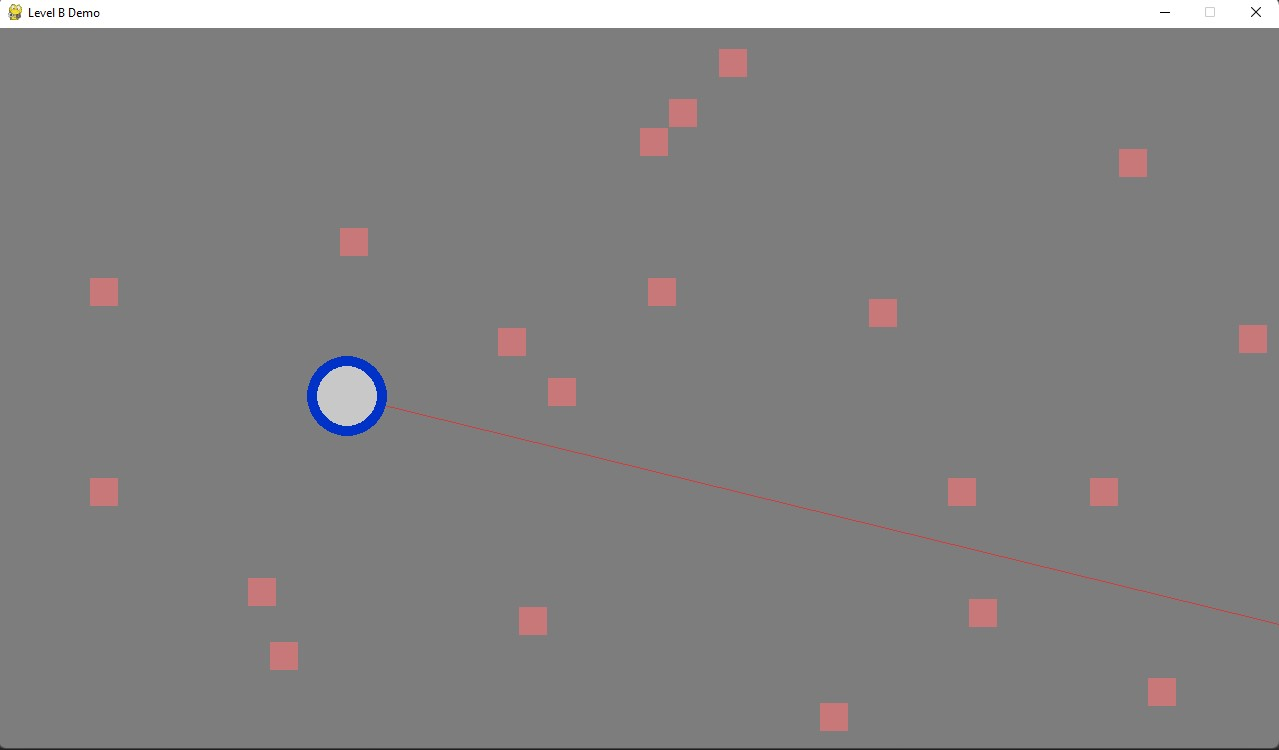
\includegraphics[width=8cm]{Level B Demo2}\\[1cm]
\\
This code snippet shows the object oriented programming and the hierarchy of classes and objects. The Entity class includes both the Player and Enemy classes as its children. The enemy class also contains code for random movement (see more in GitHub).

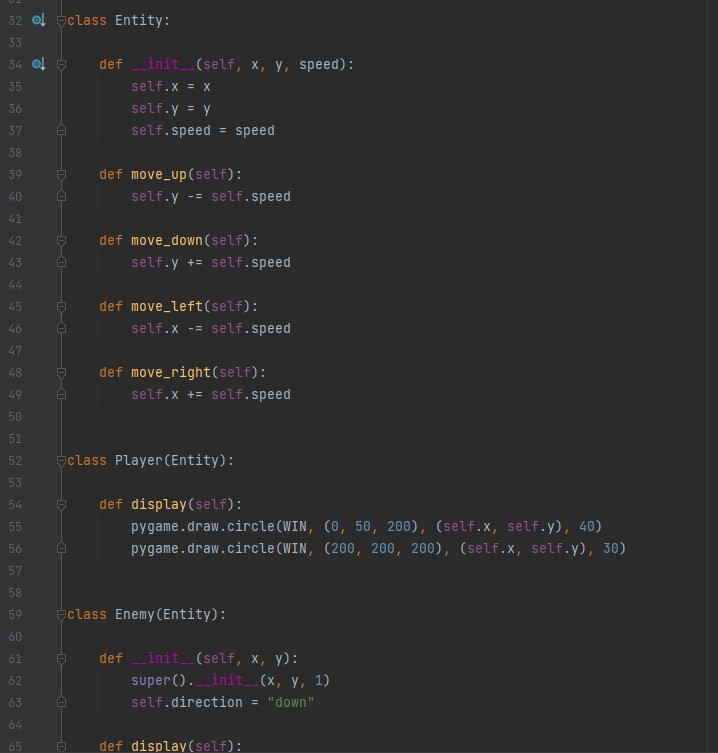
\includegraphics[width=8cm]{Level B Demo Code1}\\[1cm]
\\

These two code snippets shows the Game class being the main class which handles all the events.

\begin{figure}[!htb]%
    \centering
    \subfloat[\centering Code showing Game class]{{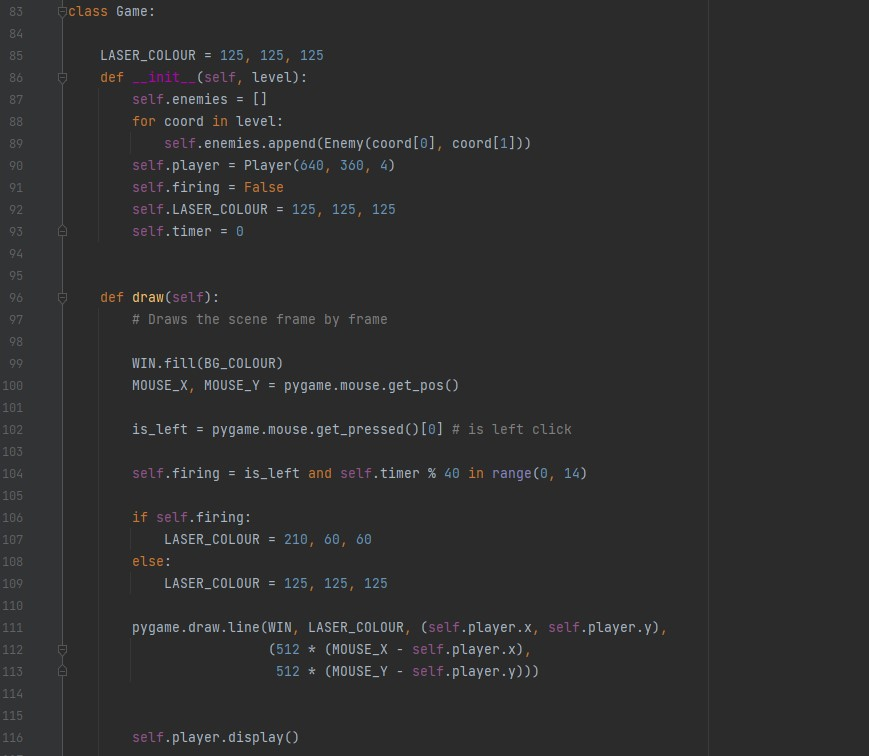
\includegraphics[width=6.5cm]{Level B Demo Code2} }}%
    \qquad
    \subfloat[\centering Code showing how enemies work]{{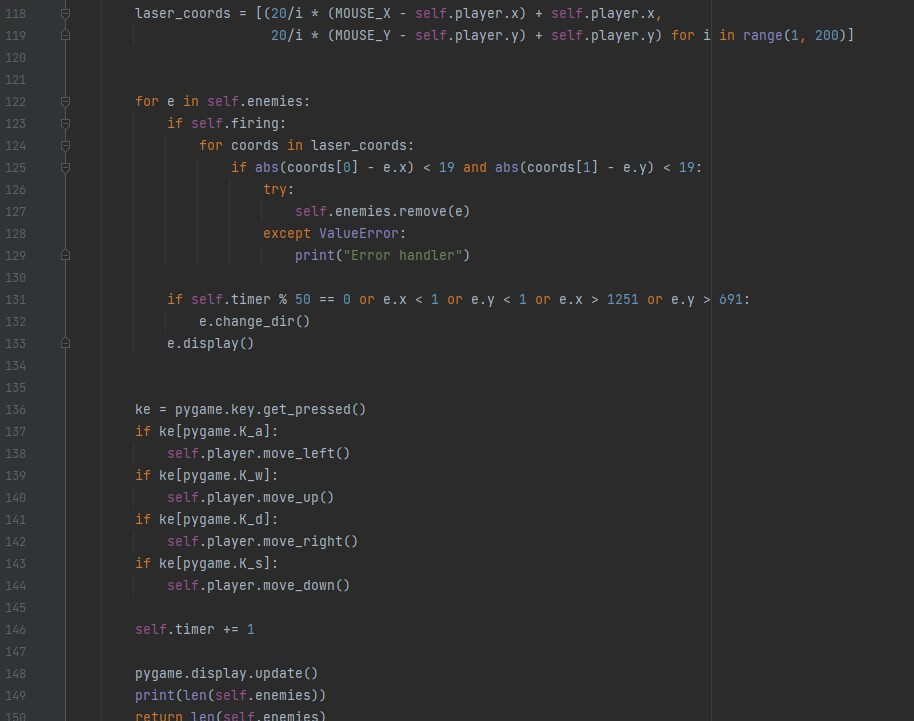
\includegraphics[width=6.5cm]{Level B Demo Code3} }}%
\end{figure}


%=============================================================================

\newpage
\section{Level C: Deeper Understanding}

Level C focuses on showing that you have actually understood the tool or technology at a relatively advanced level. You will need to compare it to alternatives, identifying key strengths and weaknesses, and the areas where this tool is most effective. 

\subsection{Strengths}
What are the key strengths of the item you have learnt? (50-100 words)

\subsection{Weaknesses}
What are the key weaknesses of the item you have learnt? (50-100 words)

\subsection{Usefulness}
Describe one scenario under which you believe the topic you have learnt could be useful. (50-100 words)

\subsection{Key Question 1}
Note: This question is in the table in the ‘Self Learning: List of Topics’ page on Canvas. (50-100 words)

\subsection{Key Question 2}
Note: This question is in the table in the ‘Self Learning: List of Topics’ page on Canvas. (50-100 words)


%=============================================================================

\newpage
\section{Level D: Evolution of skills}
\vspace{5mm}
\subsection{Level D Demonstration}

This is a short description of the application that you have developed. (50-100 words).
\textit{{\bf IMPORTANT:} You might wish to submit this as part of an earlier submission in order to obtain feedback as to whether this is likely to be acceptable for level D.}

\subsection{Application artifacts}

Include here a description of what you actually created (what does it do? How does it work? How did you create it?). Include any code or other related artefacts that you created (these should also be included in your github repository).

If you do include screengrabs to show what you have done then these should be annotated to explain what it is showing and what the application does.

\subsection{Alternative tools/technologies}
Identify 2 alternative tools/technologies that can be used instead of the one you studied for your topic. (e.g. if your topic was Python, then you might identify Java and Golang)
\subsection{Comparative Analysis}
Describe situations in which both your topic and each of the identified alternatives would be preferred over the others (100-200 words).



%=============================================================================

\newpage

\bibliographystyle{ieeetran}
\bibliography{main}

\end{document}
\end{report}
